\documentclass[11pt,a4paper]{article}

\usepackage[margin=2.4cm]{geometry}
\usepackage{amsmath,amssymb}
\usepackage{graphicx}
\usepackage{booktabs}
\usepackage{caption}
\usepackage[table]{xcolor}
% microtype removed: on this TeX Live build its \AtBeginDocument hook
% stalls the run indefinitely for this document under both pdflatex and
% xelatex. It only affects micro-typography, so dropping it costs nothing
% substantive.
\usepackage{enumitem}
% Lightweight stand-in for siunitx: this document only needs "number
% thin-space unit", and siunitx's expl3 machinery stalls the run on this
% TeX Live build.
\newcommand{\qty}[2]{#1\,#2}
\usepackage{float}
% Seven full-width floats in a 10-page document will thrash the placement
% algorithm and can stall the run outright at \end{document}, when every
% deferred float competes at once.  Loosen the fraction limits and allow more
% floats per page so each one places on its first attempt.
\renewcommand{\topfraction}{0.92}
\renewcommand{\bottomfraction}{0.80}
\renewcommand{\textfraction}{0.06}
\renewcommand{\floatpagefraction}{0.75}
\setcounter{topnumber}{3}
\setcounter{bottomnumber}{2}
\setcounter{totalnumber}{5}
\usepackage[colorlinks=true,linkcolor=accent,citecolor=accent,urlcolor=accent]{hyperref}

\definecolor{accent}{HTML}{2563EB}
\definecolor{warn}{HTML}{DC2626}
\definecolor{muted}{HTML}{64748B}
\definecolor{ink}{HTML}{18181B}
\definecolor{rowtint}{HTML}{F4F4F5}

\captionsetup{font=small, labelfont={bf,color=ink}, width=0.92\textwidth}
\setlist[itemize]{itemsep=2pt, topsep=4pt}

\newcommand{\MEAS}{\textcolor{accent}{\textsc{measured}}}
\newcommand{\REV}{\textcolor{ink}{\textsc{review}}}
\newcommand{\DAT}{\textcolor{ink}{\textsc{datasheet}}}
\newcommand{\LIT}{\textcolor{muted}{\textsc{literature}}}
\newcommand{\ASS}{\textcolor{warn}{\textsc{assumed}}}

\title{\bfseries Airflow and Thermal Model of the CalSol Excalibur Battery Box}
\author{Reduced-order analysis from the \texttt{Main Battery} CAD}
\date{\today}

\begin{document}
\maketitle

\begin{abstract}
\noindent
A reduced-order airflow and thermal model of the CalSol Excalibur battery
enclosure, built on geometry measured directly from the \texttt{Main Battery}
STEP export rather than reconstructed. The pack is a staggered bank of
408 LG INR18650 MJ1 cells cooled by \qty{80}{mm} fans mounted in
two rectangular cutouts on opposite ends of the box.

Three results stand out. First, the cell bank accounts for \qty{97.7}{\%}
of the system resistance and the fans sit at \qty{99}{\%} of their
dead-head pressure, so \emph{adding fans in parallel is nearly useless}: going
from three to twelve buys \qty{0.10}{\textdegree C} for \qty{227}{W}. Second,
staging fans \emph{in series} --- pushing at one cutout and pulling at the other
--- raises the flow from \qty{93.2}{CFM} to \qty{131.6}{CFM} and drops the hottest
cell from \qty{47.02}{\textdegree C} to \qty{45.12}{\textdegree C} at identical power,
essentially reaching the \qty{45}{\textdegree C} design goal with no change to the
hardware. Third, a configuration of one fan on each face is both cooler and
cheaper than the current three-on-one-face arrangement
(\qty{46.18}{\textdegree C} at \qty{50.4}{W} against \qty{47.02}{\textdegree C} at
\qty{75.6}{W}).

A transient lumped-node model with seeded manufacturing scatter is included,
along with an explicit statement of where the model's assumptions are weakest.
\end{abstract}

\section{Geometry}

All geometry is read from \texttt{fullbatterybox/Main Battery.step}
(\qty{57}{MB}, 3374 solids) through the OpenCASCADE XCAF reader,
which preserves part names and colours from the assembly tree. Bodies are
classified by CAD part name; the 408 cells are identified by name and
confirmed by shape.

\begin{table}[htbp]
\centering
\caption{Pack geometry, measured from the STEP. The cell diameter is taken from
the \emph{cylindrical face} rather than the bounding box: the box reads
\qty{19.92}{mm} because it includes the terminal button, and that
difference moves the inter-cell gap from \qty{0.58}{mm} to
\qty{2.10}{mm} --- a factor of 3.6 in the quantity that sets the
pressure drop.}
\label{tab:geom}
\small
\begin{tabular}{llr}
\toprule
\textbf{Quantity} & \textbf{Symbol} & \textbf{Value} \\
\midrule
Cells & $N$ & 408 \\
Arrangement & --- & $17 \times 12 \times 2$, staggered \\
Cell diameter & $D$ & \qty{18.40}{mm} \\
Cell length & $L$ & \qty{65.00}{mm} \\
Transverse pitch & $S_T$ & \qty{20.50}{mm} \\
Longitudinal pitch & $S_L$ & \qty{25.20}{mm} \\
Diagonal pitch & $S_D$ & \qty{27.20}{mm} \\
Minimum gap & $S_T - D$ & \qty{2.10}{mm} \\
Free-area ratio & $A_{\min}/A_{\mathrm{face}}$ & 0.1024 \\
Bank frontal face & --- & \qty{246.0}{mm} $\times$ \qty{130.0}{mm} \\
Total wetted area & $A_{\mathrm{tot}}$ & \qty{1.533}{m$^2$} \\
\bottomrule
\end{tabular}
\end{table}

\subsection{The openings}

The enclosure is pierced by two large rectangular cutouts on opposite ends of
the $z$ axis, \qty{590}{mm} apart, with the cell block centred between
them. \texttt{Battery Box.step} is the only file in the set exported with true
B-rep solids, so the cutouts could be measured as inner wires on planar faces
rather than estimated.

\begin{table}[htbp]
\centering
\caption{Measured openings. Each fits exactly three \qty{80}{mm} fan
frames across its width, independently confirming the design review's
``3 across the pack''. The rear cutout is partly blocked by an internal truss.}
\label{tab:openings}
\small
\begin{tabular}{llrrr}
\toprule
\textbf{Opening} & \textbf{CAD part} & \textbf{Size} & \textbf{Porosity} & \textbf{Free area} \\
\midrule
Blue, front & \texttt{Front Plate-1} & 251.3 $\times$ \qty{121.0}{mm} & 1.000 & \qty{304.1}{cm$^2$} \\
Green, rear & \texttt{Rear Plate-1} & 244.0 $\times$ \qty{124.0}{mm} & 0.886 & \qty{268.1}{cm$^2$} \\
Front duct & \texttt{Front Duct-1} & 247.3 $\times$ \qty{117.0}{mm} & 1.000 & \qty{289.3}{cm$^2$} \\
\bottomrule
\end{tabular}
\end{table}

The blue cutout is \qty{251.3}{mm} wide against a bank face of
\qty{246.0}{mm}: a \qty{2}{\%} match. The openings were sized to
the bank, which fixes the flow axis as $z$ --- air crosses the 17 rows.

\begin{figure}[htbp]
\centering
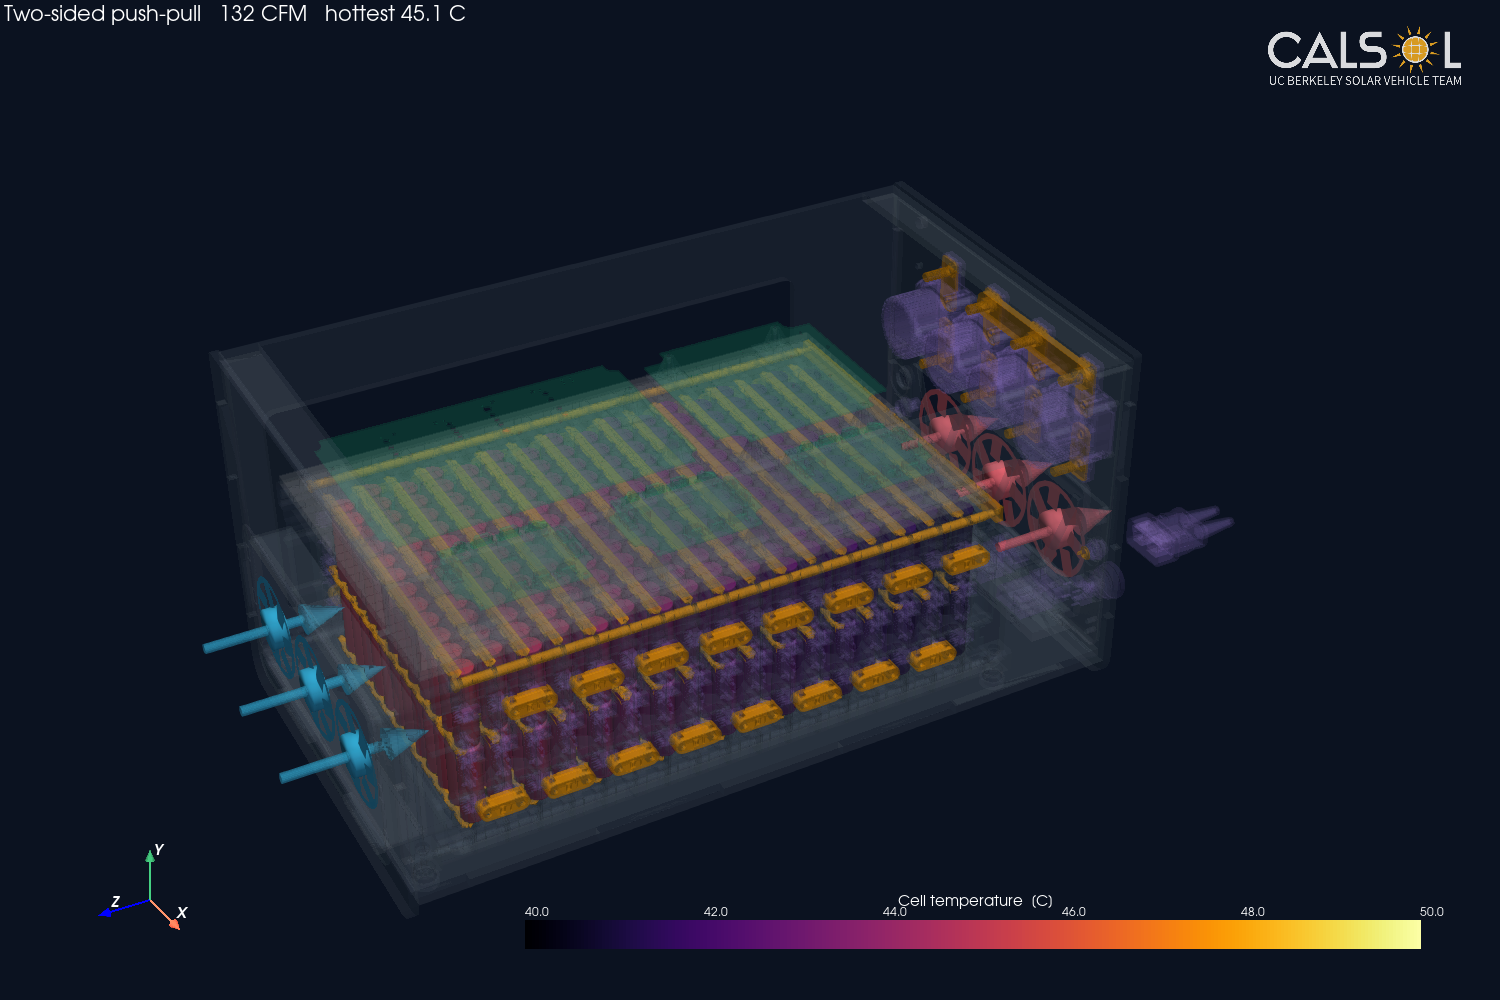
\includegraphics[width=0.84\textwidth]{figs/render_twosided.png}
\caption{The assembly as modelled, with the enclosure drawn translucent. Blue
glyphs are intake fans at the \texttt{Front Plate} cutout, red are exhaust at
the \texttt{Rear Plate}; cells are coloured by computed temperature. The purple
bodies at the far end are the four Gigavac GX11 contactors.}
\label{fig:render}
\end{figure}

\section{Governing equations}

\subsection{Pressure drop and the operating point}

The bank drop follows the Žukauskas correlation for staggered tube banks,
\begin{equation}
\Delta p_{\mathrm{bank}} \;=\; N_L \, \chi \, f \, \frac{\rho V_{\max}^{2}}{2},
\label{eq:dpbank}
\end{equation}
where $V_{\max}$ is the velocity in the minimum free area, obtained from
continuity,
\begin{equation}
V_{\max} \;=\; V_{\infty}\,\frac{S_T}{\min\!\left(S_T - D,\; 2(S_D - D)\right)}.
\label{eq:vmax}
\end{equation}
For this pack the transverse plane binds and $V_{\max} = 9.76\,V_{\infty}$. The
operating point is the flow at which the fan characteristic meets the system
resistance,
\begin{equation}
\Delta p_{\mathrm{fan}}(Q) \;=\; \Delta p_{\mathrm{sys}}(Q)
\;=\; \Delta p_{\mathrm{bank}}(Q) + \Delta p_{\mathrm{duct}}(Q),
\label{eq:op}
\end{equation}
solved by Brent's method with the air state iterated to consistency, since
density depends on how much the air has warmed and that depends on the flow.

\subsection{Fan composition: the central result}

Fans side by side on one face are in \emph{parallel} --- equal pressure, flows
add:
\begin{equation}
Q(\Delta p) \;=\; \sum_i Q_i(\Delta p).
\label{eq:parallel}
\end{equation}
Fans on opposite faces of the same duct are in \emph{series} --- equal flow,
pressures add:
\begin{equation}
\boxed{\;\sum_i \Delta p_i(Q) \;=\; \Delta p_{\mathrm{sys}}(Q).\;}
\label{eq:series}
\end{equation}
Which law applies is the difference between a useful fan and a wasted one, for
the reason developed in \S\ref{sec:fans}.

Continuity over the box closes the system:
\begin{equation}
\sum_{i \in \mathrm{inlets}} Q_i \;=\; \sum_{j \in \mathrm{outlets}} Q_j .
\label{eq:continuity}
\end{equation}
Equation~\eqref{eq:continuity} has no solution for $Q > 0$ if every opening
carries a fan blowing inward: the box simply pressurises until one face
reverses. The implementation raises an error in that case rather than returning
a plausible number.

\subsection{Heat transfer}

The convective coefficient comes from the Žukauskas correlation,
\begin{equation}
\mathrm{Nu} \;=\; C_1 C_2 \, \mathrm{Re}_{\max}^{m} \, \mathrm{Pr}^{0.36}
\left(\frac{\mathrm{Pr}}{\mathrm{Pr}_s}\right)^{1/4},
\qquad h \;=\; \frac{\mathrm{Nu}\,k}{D},
\label{eq:nu}
\end{equation}
with $C_1$ a function of $S_T/S_L$ and $C_2$ the shallow-bank correction. Air
is marched row by row, its properties re-evaluated at each row's local
temperature:
\begin{equation}
\dot m \, c_p \, \Delta T_{\mathrm{air},r} \;=\; \sum_{i \in r} \dot Q_i,
\qquad
T_{\mathrm{cell},i} \;=\; T_{\mathrm{air},r(i)} + \frac{\dot Q_i}{h A_i}.
\label{eq:march}
\end{equation}

\subsection{Transient model}

For time-dependent behaviour each cell becomes a lumped node of capacity
$C_i = m c_p$, coupled to its neighbours by conduction and to the local air by
convection:
\begin{equation}
C_i \frac{\mathrm{d}T_i}{\mathrm{d}t}
\;=\; \dot q_i
\;-\; h_i A_i \left(T_i - T_{\mathrm{air},r(i)}\right)
\;+\; \sum_{j \in \mathcal{N}(i)} G_{ij}\left(T_j - T_i\right).
\label{eq:transient}
\end{equation}
Manufacturing spread enters physically, through the cell properties rather than
as noise added to the result:
\begin{equation}
\dot q_i = I_{\mathrm{cell}}^{2} R_i,
\qquad R_i = R_{\mathrm{int}}\left(1 + \epsilon_i\right),
\qquad \epsilon_i \sim \mathcal{N}\!\left(0, \sigma_R^{2}\right),
\label{eq:scatter}
\end{equation}
drawn once from a seeded generator so a run is reproducible.

Equation~\eqref{eq:transient} is integrated with explicit Euler. Stability
requires
\begin{equation}
\Delta t \;<\; \min_i \frac{C_i}{h_i A_i + \sum_j G_{ij}} \;=\; \qty{29.3}{s},
\label{eq:cfl}
\end{equation}
so the chosen $\Delta t = \qty{0.5}{s}$ carries a 59$\times$ margin.
The system is not stiff --- convection dominates conduction by roughly an order
of magnitude --- so an implicit scheme would cost a dense solve per step and buy
nothing. The air is treated as quasi-steady: its transit time through the bank
is \qty{0.31}{s} against a cell time constant of \qty{39.9}{s}, a
separation of 128$\times$.

\section{Operating conditions}

\begin{table}[htbp]
\centering
\caption{Inputs, each tagged with its provenance. Nothing here is invented;
where a value could not be sourced it is marked \ASS\ and surfaced in the tool.}
\label{tab:inputs}
\small
\rowcolors{2}{rowtint}{white}
\begin{tabular}{llr l}
\toprule
\textbf{Parameter} & \textbf{Symbol} & \textbf{Value} & \textbf{Source} \\
\midrule
Pack configuration & --- & 34S12P & \REV \\
Cell internal resistance & $R_{\mathrm{int}}$ & \qty{28}{m$\Omega$} & \REV \\
Pack voltage & $V$ & \qty{85}{V} & \REV \\
Worst-case draw & $P$ & \qty{5200}{W} & \REV \\
Pack current & $I$ & \qty{61.18}{A} & derived \\
Cell current & $I_{\mathrm{cell}}$ & \qty{5.10}{A} & derived \\
Pack heat load & $\dot Q$ & \qty{296.9}{W} & derived \\
Per-cell heat & $\dot q$ & \qty{0.728}{W} & derived \\
Inlet air temperature & $T_\infty$ & \qty{40}{\textdegree C} & \REV \\
Design goal & --- & \qty{45}{\textdegree C} & \REV \\
Absolute limit & --- & \qty{60}{\textdegree C} & \REV \\
Fan & --- & Delta GFB0812ES-E, \qty{25.2}{W} & \DAT \\
Cell mass & $m$ & \qty{48}{g} & \DAT \\
Cell specific heat & $c_p$ & \qty{1050}{J\,kg$^{-1}$K$^{-1}$} & \LIT \\
Radial conductivity & $k_r$ & \qty{0.5}{W\,m$^{-1}$K$^{-1}$} & \LIT \\
Cell--cell conductance & $G$ & \qty{0.02}{W/K} & \ASS \\
Resistance scatter & $\sigma_R$ & \qty{5}{\%} & \ASS \\
Duct + grille loss & $K$ & $3.5 + 1.4$ & \ASS \\
Contactor + PCB heat & --- & \qty{32.5}{W} & \ASS \\
\bottomrule
\end{tabular}
\end{table}

\section{Results}

\subsection{Why more fans do not help}
\label{sec:fans}

At the one-sided operating point the bank contributes \qty{1421.9}{Pa} of a
\qty{1454.9}{Pa} total --- \qty{97.7}{\%}. The fan is delivering
\qty{148}{mmH$_2$O} against a dead-head of
\qty{150}{mmH$_2$O}, which is to say it is operating on the flat,
near-vertical part of its curve. Adding fans in parallel adds flow capacity
where the curve has already collapsed.

\begin{table}[htbp]
\centering
\caption{Fan count against outcome, both candidate flow axes. On the axis the
real cutouts occupy, a four-fold increase in fan power is worth
\qty{0.10}{\textdegree C}.}
\label{tab:fancount}
\small
\begin{tabular}{r rr rr}
\toprule
& \multicolumn{2}{c}{\textbf{flow $\parallel z$ (cutout axis)}}
& \multicolumn{2}{c}{\textbf{flow $\parallel x$ (open axis)}} \\
\cmidrule(lr){2-3}\cmidrule(lr){4-5}
\textbf{Fans} & \textbf{Flow} & \textbf{Hottest cell} & \textbf{Flow} & \textbf{Hottest cell} \\
\midrule
1  & \qty{78.6}{CFM} & \qty{48.21}{\textdegree C} & \qty{126.3}{CFM} & \qty{47.08}{\textdegree C} \\
3  & \qty{93.2}{CFM} & \qty{47.02}{\textdegree C} & \qty{359.7}{CFM} & \qty{43.01}{\textdegree C} \\
6  & \qty{94.4}{CFM} & \qty{46.94}{\textdegree C} & \qty{613.5}{CFM} & \qty{41.97}{\textdegree C} \\
12 & \qty{94.7}{CFM} & \qty{46.92}{\textdegree C} & \qty{817.2}{CFM} & \qty{41.58}{\textdegree C} \\
\bottomrule
\end{tabular}
\end{table}

\begin{figure}[htbp]
\centering
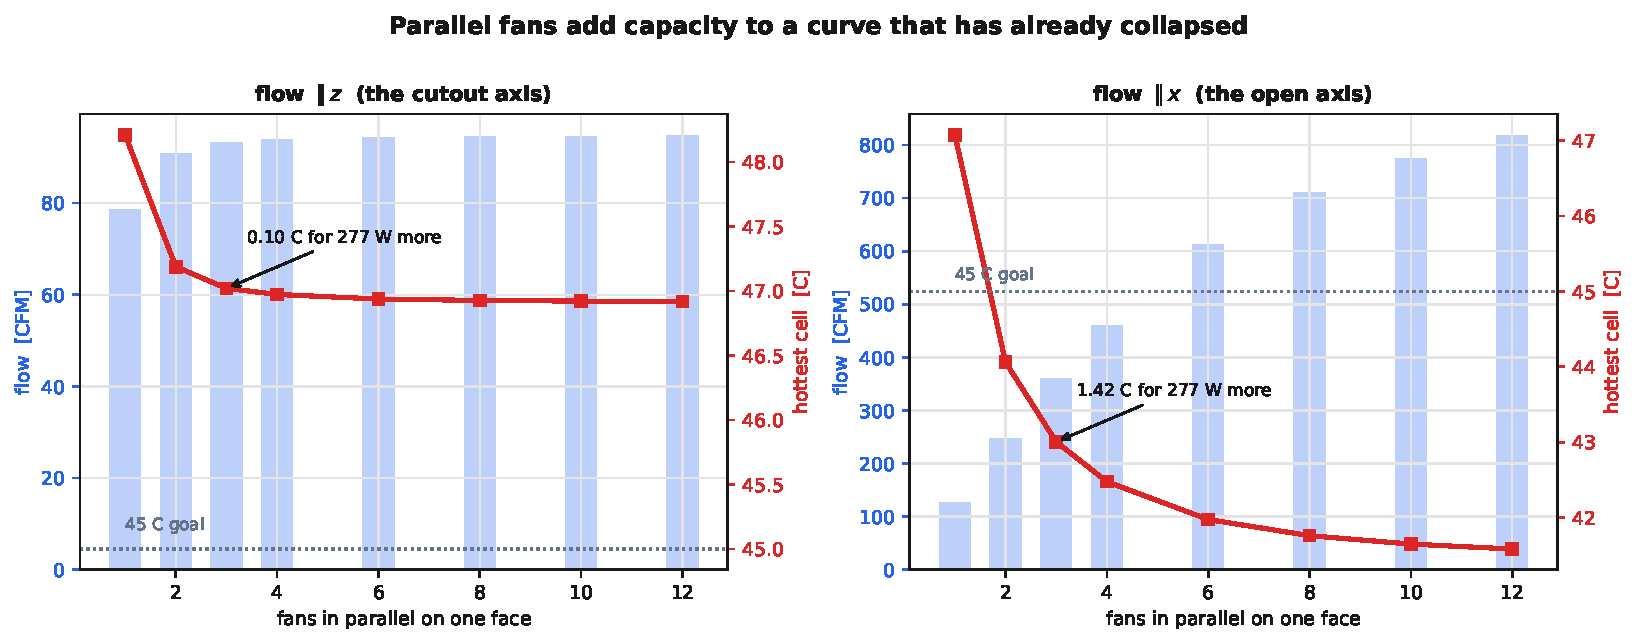
\includegraphics[width=\textwidth]{figs/fan_count.pdf}
\caption{The same fans on the two candidate axes. On the cutout axis (left) the
curve is flat in fan count; on the open axis (right) the same hardware more than
doubles the flow. The difference is the free-area ratio: 0.102 against
0.349.}
\label{fig:fancount}
\end{figure}

\subsection{Series staging}

Pushing at one cutout while pulling at the other puts the two fan sets in
series, so by \eqref{eq:series} their pressure rises add. The system curve is
unchanged; the available pressure is doubled, and the intersection moves.

\begin{figure}[htbp]
\centering
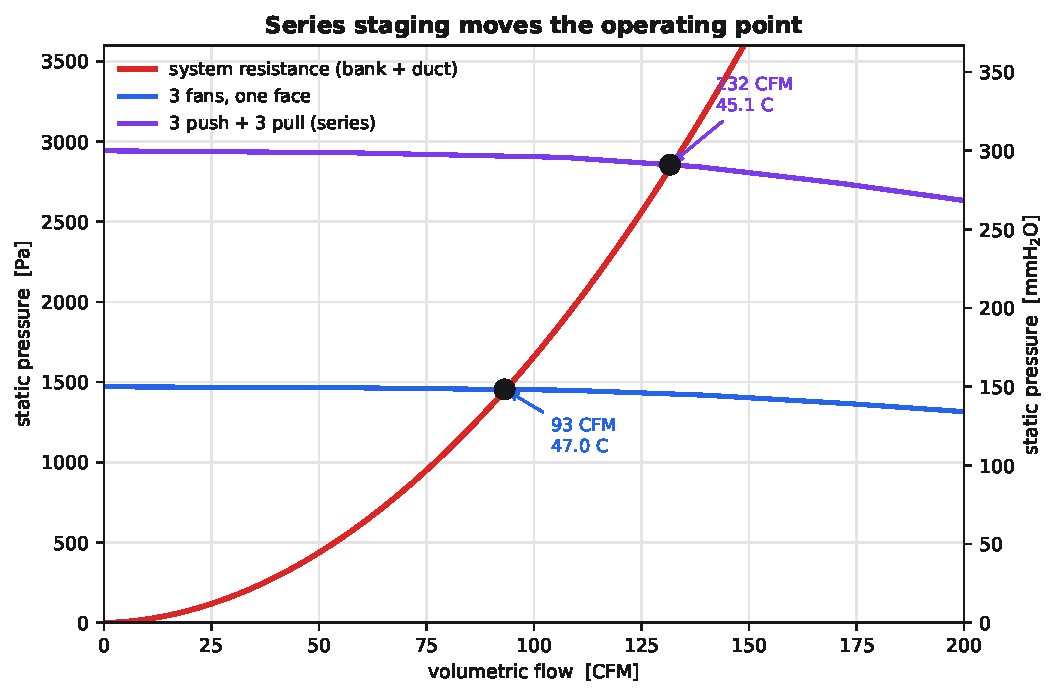
\includegraphics[width=0.84\textwidth]{figs/network.pdf}
\caption{Fan characteristics against the system resistance. The red curve is
the same in both cases --- only the available pressure differs. Series staging
moves the operating point from \qty{93}{CFM} to \qty{132}{CFM}.}
\label{fig:network}
\end{figure}

\begin{table}[htbp]
\centering
\caption{One-sided against push--pull at identical fan power.}
\label{tab:pp}
\small
\begin{tabular}{lrr}
\toprule
\textbf{Quantity} & \textbf{3 fans, one face} & \textbf{3 push + 3 pull} \\
\midrule
Flow                      & \qty{93.2}{CFM}    & \qty{131.6}{CFM} \\
Face velocity             & \qty{1.38}{m/s} & \qty{1.94}{m/s} \\
$V_{\max}$                & \qty{13.43}{m/s} & \qty{18.96}{m/s} \\
$\mathrm{Re}_{\max}$      & 14373       & 20391 \\
$h$                       & \qty{136.7}{W\,m$^{-2}$K$^{-1}$} & \qty{168.3}{W\,m$^{-2}$K$^{-1}$} \\
$\Delta p$ bank           & \qty{1422}{Pa} & \qty{2789}{Pa} \\
$\Delta p$ total          & \qty{1455}{Pa} & \qty{2855}{Pa} \\
Air temperature rise      & \qty{5.95}{\textdegree C} & \qty{4.21}{\textdegree C} \\
Exhaust air               & \qty{45.95}{\textdegree C} & \qty{44.21}{\textdegree C} \\
\textbf{Hottest cell}     & \textbf{\qty{47.02}{\textdegree C}} & \textbf{\qty{45.12}{\textdegree C}} \\
Fan power                 & \qty{75.6}{W}  & \qty{151.2}{W} \\
\bottomrule
\end{tabular}
\end{table}

\begin{figure}[htbp]
\centering
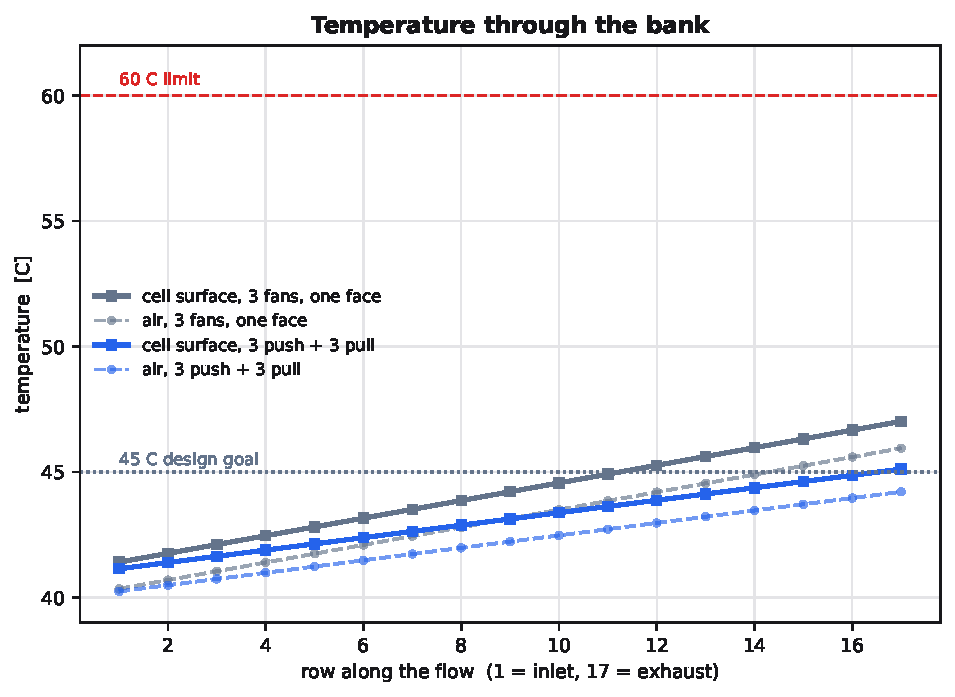
\includegraphics[width=0.78\textwidth]{figs/march.pdf}
\caption{Air and cell temperature along the flow. Push--pull both lowers the
whole profile and flattens it, because the larger mass flow cuts the air-side
rise from \qty{5.95}{\textdegree C} to \qty{4.21}{\textdegree C}.}
\label{fig:march}
\end{figure}

\subsection{Placement search}

All 30 physically realisable arrangements over the two cutouts were
enumerated --- each face either unused, blowing in, or drawing out, with up to
three fans, subject to at least one path in and one out. Each costs a single
root find, so exhaustive enumeration is both cheaper than an optimiser and
provably optimal within the space.

\begin{figure}[htbp]
\centering
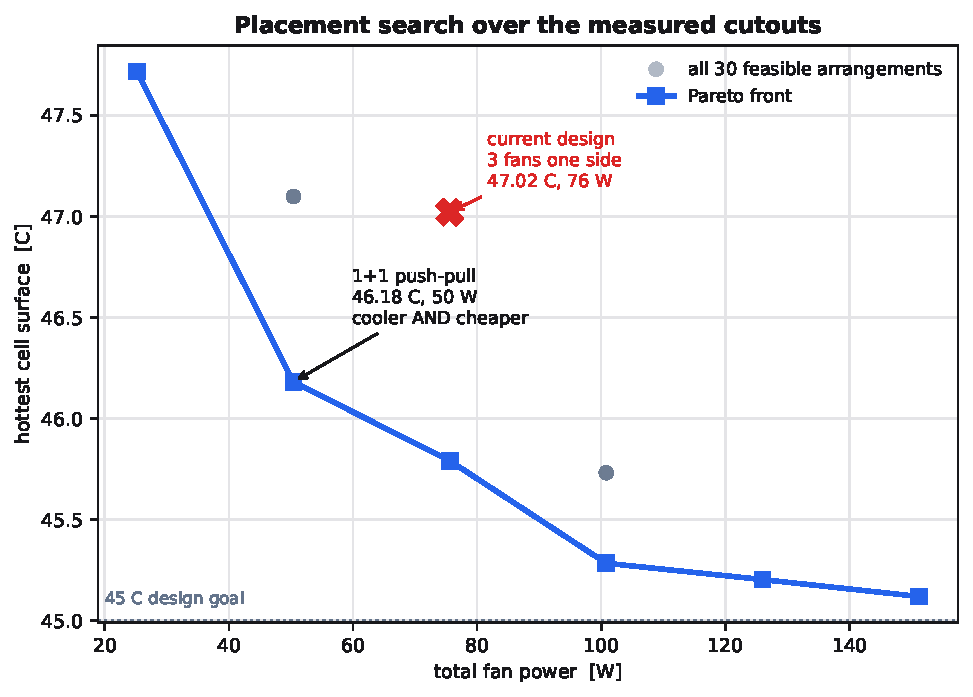
\includegraphics[width=0.84\textwidth]{figs/pareto.pdf}
\caption{Peak cell temperature against fan power. The current design (red
cross) is \emph{dominated}: one fan on each face is both cooler and cheaper.}
\label{fig:pareto}
\end{figure}

\begin{table}[htbp]
\centering
\caption{Pareto front. Most of the available benefit arrives with the first fan
on the second face, not with more fans on the first.}
\label{tab:pareto}
\small
\begin{tabular}{lrrr}
\toprule
\textbf{Arrangement} & \textbf{Flow} & \textbf{Hottest cell} & \textbf{Power} \\
\midrule
1 green in                 & \qty{84.1}{CFM}  & \qty{47.72}{\textdegree C} & \qty{25.2}{W} \\
1 blue in + 1 green out    & \qty{107.1}{CFM} & \qty{46.18}{\textdegree C} & \qty{50.4}{W} \\
1 blue in + 2 green out    & \qty{115.0}{CFM} & \qty{45.79}{\textdegree C} & \qty{75.6}{W} \\
2 blue in + 2 green out    & \qty{127.1}{CFM} & \qty{45.28}{\textdegree C} & \qty{100.8}{W} \\
2 blue in + 3 green out    & \qty{129.3}{CFM} & \qty{45.20}{\textdegree C} & \qty{126.0}{W} \\
3 blue in + 3 green out    & \qty{131.6}{CFM} & \qty{45.12}{\textdegree C} & \qty{151.2}{W} \\
\midrule
\textit{current: 3 one side} & \qty{93.2}{CFM} & \qty{47.02}{\textdegree C} & \qty{75.6}{W} \\
\bottomrule
\end{tabular}
\end{table}

\subsection{Transient behaviour}

\begin{figure}[htbp]
\centering
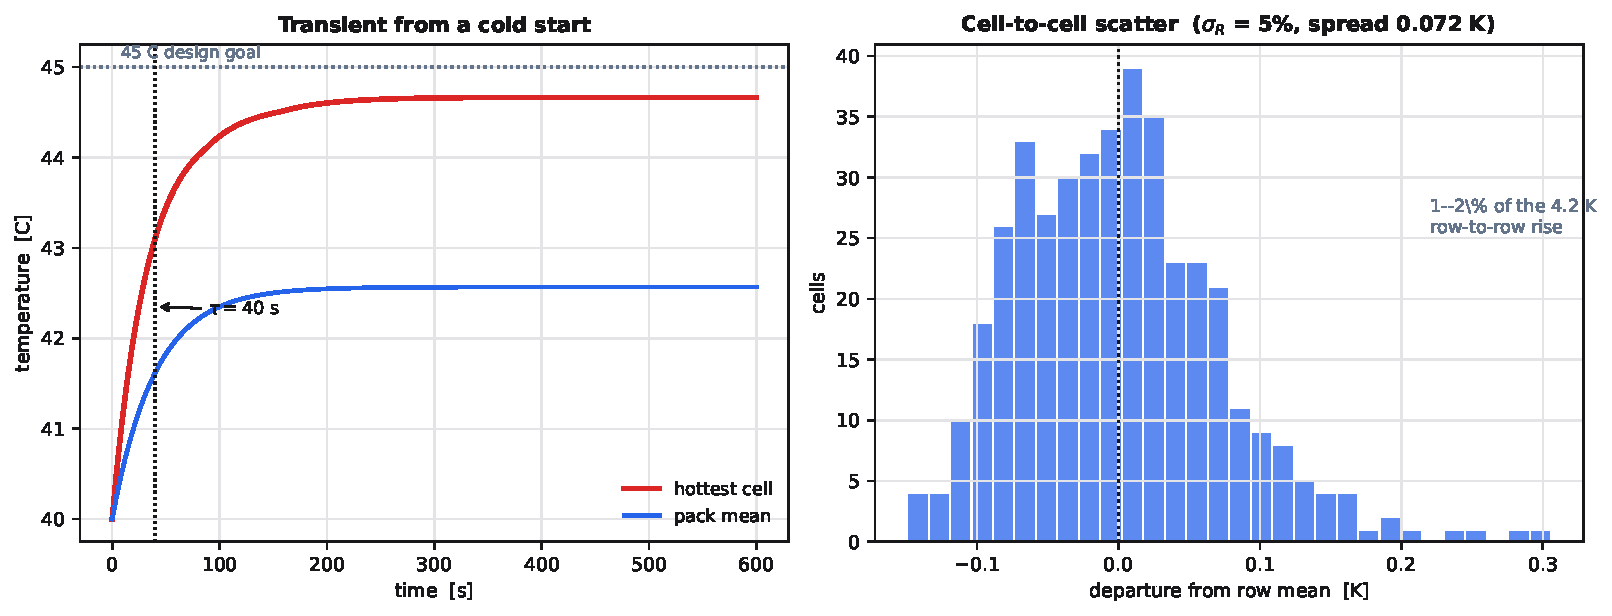
\includegraphics[width=\textwidth]{figs/transient.pdf}
\caption{Left: approach to steady state from a cold start under push--pull,
with the time constant $\tau = C/(hA) = \qty{39.9}{s}$ marked. Right: the
distribution of each cell's departure from its own row mean.}
\label{fig:transient}
\end{figure}

The pack reaches \qty{99}{\%} of its final rise in roughly $5\tau \approx
\qty{200}{s}$. At $\sigma_R = \qty{5}{\%}$ the cell-to-cell spread is
\qty{-0.15--0.31}{K} about each row mean --- between 1 and
\qty{2}{\%} of the \qty{4.2}{K} row-to-row rise. \emph{The scatter is
therefore nearly invisible against the axial gradient}, which is worth stating
plainly: a visualisation that makes it look dramatic is exaggerating. The tool
exposes a separate gain control for that purpose, labelled as non-physical.

\section{Verification}

\begin{table}[htbp]
\centering
\caption{Checks run against the implementation.}
\label{tab:verif}
\small
\begin{tabular}{ll}
\toprule
\textbf{Check} & \textbf{Result} \\
\midrule
Network model reproduces the single-fan solver & exact, \qty{0.0}{CFM} difference \\
Transient $t \to \infty$ against analytic steady state & \qty{2.8e-12}{K} \\
Exponential approach at $t = \tau$ & 0.6336 vs $1 - e^{-1} = 0.6321$ \\
Transient energy balance & 1.1e-15 relative \\
Steady energy balance & $< 1e-3$ relative \\
$\mathrm{Re}_{\max}$ within Žukauskas validity & 14373--20391 \\
Cells recovered from CAD & 408 \\
Both-inlet topology & raises, does not return a value \\
\bottomrule
\end{tabular}
\end{table}

Against the design review's own MATLAB study the model runs
\qty{11--22}{\%} hotter across five published operating points. The
bias is consistent and traceable to the friction extrapolation described below;
it is conservative.

\section{Limitations}

These are stated in order of how much they matter.

\begin{enumerate}[leftmargin=*]
\item \textbf{The friction extrapolation dominates everything.} The bank is
\qty{97.7}{\%} of the system resistance, and its friction factor is
extrapolated from the tightest published Žukauskas curve ($P_T = 1.25$) to the
actual $P_T = 1.114$. Every pressure and flow in this report inherits that
extrapolation. It over-predicts $\Delta p$ and so under-predicts flow.

\item \textbf{The lumped-node assumption is formally violated.} With
$\mathrm{Bi} = h(D/4)/k_r = 1.55$, well above the usual 0.1
threshold, a node temperature is a \emph{volume mean}, not a surface
temperature. The centre-to-surface rise is \qty{1.78}{K} --- larger than
the entire scatter effect --- and is added explicitly before any comparison with
the \qty{60}{\textdegree C} surface limit.

\item \textbf{Several inputs are assumptions, not measurements.} The cell--cell
conductance (\qty{0.02}{W/K}) is the weakest and the first worth
measuring. Contactor and PCB dissipation (\qty{32.5}{W}) does not appear in
the design review at all; because those bodies sit outside the cell air path it
raises the exhaust by \qty{0.46}{K} and leaves cell temperatures untouched.

\item \textbf{One-dimensional flow.} Uniform velocity across the face, no
bypass around the bank, no recirculation, and heat spread evenly over the cells.
Real packs leak around the edges, which would penalise the low-resistance
configurations more than the high-resistance ones.

\item \textbf{The push--pull result is unvalidated.} No CFD or experimental
data exists for it. The series composition assumes the two fan sets do not
interfere aerodynamically --- reasonable at \qty{590}{mm} separation
with the bank between them, but unverified.

\item \textbf{The flow direction is a modelling choice.} The fans and ducts were
suppressed before the CAD export, so nothing in the geometry proves which way
the air actually moves. The cutout dimensions make the $z$ axis overwhelmingly
likely, and that is what is modelled throughout.
\end{enumerate}

\section{Conclusions}

\begin{itemize}
\item The pack passes the \qty{60}{\textdegree C} limit in every configuration
examined, with at least \qty{11.8}{\textdegree C} of margin.
\item The current three-fans-on-one-face arrangement reaches
\qty{47.02}{\textdegree C} and misses the \qty{45}{\textdegree C} design goal by
\qty{2.02}{\textdegree C}.
\item \textbf{Moving one of those fans to the opposite cutout is cooler and
cheaper} --- \qty{46.18}{\textdegree C} at \qty{50.4}{W} with one fan per face.
Running three on each face reaches \qty{45.12}{\textdegree C} and effectively meets
the goal.
\item Adding fans to a single face is not a useful lever. The bank, not the
fans, sets the flow.
\item The largest single uncertainty is the friction extrapolation. If one
measurement is to be made, a pressure-drop test across the bank at a known flow
would retire most of the doubt in this report.
\end{itemize}

\end{document}
